% Appendix. Assemble on Day 12.
\chapter{Appendix}
\label{ch:appendix}

\section{Additional Tables}
\label{app:per-country}
This section collects detailed tables that support the main text: the per-maturity Phase~I estimates, the cross-country yield correlations, the in-sample subsample and inflation-measure estimates, and the Italy crisis decomposition.

\begin{table}[htbp]
  \caption{Phase~I by maturity: predicting individual excess returns with the
    cycle factor}
  \label{tab:mr-phase1-mat}
  \centering
  % mr_t1b_maturity — Phase I by maturity: individual excess returns on the cycle factor.
% Numbers transcribed from tables/mr_t1b_maturity.pdf (generated by main_results.R).
\footnotesize
\setlength{\tabcolsep}{4pt}
\begin{tabular}{l ccc ccc ccc}
  \toprule
  & \multicolumn{3}{c}{$n=2$} & \multicolumn{3}{c}{$n=5$} & \multicolumn{3}{c}{$n=10$} \\
  \cmidrule(lr){2-4}\cmidrule(lr){5-7}\cmidrule(lr){8-10}
  Country & $\hat{\beta}$ & $t$ & $R^{2}$ & $\hat{\beta}$ & $t$ & $R^{2}$ & $\hat{\beta}$ & $t$ & $R^{2}$ \\
  \midrule
  Belgium     & $0.83$ & $(4.88)$ & $0.272$ & $1.16$ & $(4.64)$ & $0.302$ & $1.01$ & $(3.96)$ & $0.251$ \\
  Germany     & $0.75$ & $(3.70)$ & $0.203$ & $1.19$ & $(4.16)$ & $0.265$ & $1.05$ & $(3.81)$ & $0.228$ \\
  France      & $0.59$ & $(2.58)$ & $0.059$ & $1.19$ & $(4.11)$ & $0.134$ & $1.22$ & $(4.84)$ & $0.149$ \\
  Italy       & $0.81$ & $(3.83)$ & $0.316$ & $1.15$ & $(4.05)$ & $0.278$ & $1.04$ & $(3.93)$ & $0.232$ \\
  Netherlands & $0.79$ & $(4.77)$ & $0.302$ & $1.19$ & $(5.51)$ & $0.358$ & $1.03$ & $(4.57)$ & $0.282$ \\
  Switzerland & $0.61$ & $(1.02)$ & $0.038$ & $1.34$ & $(1.96)$ & $0.092$ & $1.05$ & $(1.61)$ & $0.059$ \\
  United Kingdom & $0.74$ & $(3.71)$ & $0.199$ & $1.19$ & $(4.28)$ & $0.269$ & $1.07$ & $(3.62)$ & $0.229$ \\
  Sweden      & $0.86$ & $(3.87)$ & $0.245$ & $1.10$ & $(3.34)$ & $0.218$ & $1.04$ & $(3.24)$ & $0.205$ \\
  Canada      & $0.87$ & $(3.85)$ & $0.268$ & $1.14$ & $(4.48)$ & $0.316$ & $0.99$ & $(3.76)$ & $0.271$ \\
  Japan       & $0.56$ & $(2.32)$ & $0.173$ & $1.23$ & $(3.10)$ & $0.238$ & $1.21$ & $(3.81)$ & $0.283$ \\
  United States & $0.75$ & $(3.35)$ & $0.233$ & $1.14$ & $(4.33)$ & $0.314$ & $1.11$ & $(5.20)$ & $0.347$ \\
  \midrule
  G10 panel   & $0.78$ & $(14.33)$ & $0.254$ & $1.16$ & $(17.26)$ & $0.274$ & $1.06$ & $(15.56)$ & $0.246$ \\
  \bottomrule
\end{tabular}
\tabnotes{The dependent variable is the duration-standardised individual
  excess return $\rx^{(n)}_{i,t+12}/n$ for $n\in\{2,5,10\}$ years. Each
  maturity block reports the regression of $\rx^{(n)}_{i,t+12}/n$ on the local
  cycle factor $\CF_{i,t}$ of \eqref{eq:cf}, as in \eqref{eq:h-local}.
  Newey--West HAC $t$-statistics (lag length as in \Cref{sec:meth-inference}) in parentheses; $R^{2}$ is
  in-sample. ``G10 panel'' pools all countries with country fixed effects. The
  table mirrors \citet{cieslak2015}, Table~4, Panel~A: a single
  return-forecasting factor prices the whole curve, with loadings
  flat-to-rising in maturity.}

\end{table}

\begin{table}[htbp]
  \caption{Cross-country correlation of the ten-year zero-coupon yield}
  \label{tab:dh-t1-corr}
  \centering
  % dh_t1_corr10y — Cross-country correlation of the 10-year zero-coupon yield.
% Numbers transcribed from tables/dh_t1_corr10y.pdf.
\small
\setlength{\tabcolsep}{4pt}
\begin{tabular}{l ccccccccccc}
  \toprule
  Country & BE & DE & FR & IT & NL & CH & GB & SE & CA & JP & US \\
  \midrule
  Belgium        & $1.00$ &        &        &        &        &        &        &        &        &        &        \\
  Germany        & $0.98$ & $1.00$ &        &        &        &        &        &        &        &        &        \\
  France         & $0.99$ & $0.99$ & $1.00$ &        &        &        &        &        &        &        &        \\
  Italy          & $0.89$ & $0.84$ & $0.88$ & $1.00$ &        &        &        &        &        &        &        \\
  Netherlands    & $0.99$ & $1.00$ & $1.00$ & $0.85$ & $1.00$ &        &        &        &        &        &        \\
  Switzerland    & $0.95$ & $0.97$ & $0.95$ & $0.81$ & $0.97$ & $1.00$ &        &        &        &        &        \\
  United Kingdom & $0.94$ & $0.96$ & $0.96$ & $0.84$ & $0.96$ & $0.90$ & $1.00$ &        &        &        &        \\
  Sweden         & $0.95$ & $0.96$ & $0.96$ & $0.90$ & $0.96$ & $0.95$ & $0.95$ & $1.00$ &        &        &        \\
  Canada         & $0.94$ & $0.97$ & $0.95$ & $0.84$ & $0.96$ & $0.95$ & $0.95$ & $0.98$ & $1.00$ &        &        \\
  Japan          & $0.91$ & $0.91$ & $0.92$ & $0.87$ & $0.90$ & $0.85$ & $0.93$ & $0.92$ & $0.89$ & $1.00$ &        \\
  United States  & $0.90$ & $0.94$ & $0.92$ & $0.75$ & $0.93$ & $0.89$ & $0.95$ & $0.91$ & $0.96$ & $0.90$ & $1.00$ \\
  \bottomrule
\end{tabular}
\tabnotes{This table reports pairwise-complete correlations of the monthly
  ten-year zero-coupon yield $y^{(10)}_t$ across countries, computed over the
  full per-country sample (see \Cref{tab:data-coverage}). Column labels are the
  ISO codes of the countries in the first column. Correlations are uniformly
  high and tightest within the euro-area bloc. After \citet{dahlquist2013},
  Table~1.}

\end{table}

\begin{table}[htbp]
  \caption{In-sample predictability across subsamples}
  \label{tab:rob-sub-is}
  \centering
  % rob_t1_sub_is — In-sample predictability across subsamples.
% Numbers transcribed from tables/rob_t1_sub_is.pdf (generated by robustness.R).
\footnotesize
\setlength{\tabcolsep}{4pt}
\begin{tabular}{l r cc cc cc cc}
  \toprule
  & & \multicolumn{2}{c}{$\rxbar\sim\CF$} & \multicolumn{2}{c}{$\rxbar\sim\GCF$}
    & \multicolumn{2}{c}{$\rxbar^{\,\mathrm{USD}}\sim\GCF$}
    & \multicolumn{2}{c}{$\rxbar^{\,\mathrm{USD}}\sim\FXGCF$} \\
  \cmidrule(lr){3-4}\cmidrule(lr){5-6}\cmidrule(lr){7-8}\cmidrule(lr){9-10}
  Subsample & Months & $R^{2}$ & $t$ & $R^{2}$ & $t$ & $R^{2}$ & $t$ & $R^{2}$ & $t$ \\
  \midrule
  Full sample                  & $412$ & $0.247$ & $(17.03)$ & $0.247$ & $(14.26)$ & $0.080$ & $(6.20)$  & $0.143$ & $(7.99)$ \\
  Pre-crisis (--2007:06)       & $210$ & $0.237$ & $(10.21)$ & $0.164$ & $(9.92)$  & $0.120$ & $(4.72)$  & $0.300$ & $(7.42)$ \\
  Financial crisis (2007--09)  & $30$  & $0.176$ & $(1.70)$  & $0.054$ & $(1.89)$  & $0.051$ & $(1.54)$  & $0.121$ & $(-2.47)$ \\
  Euro crisis (2010--12)       & $36$  & $0.506$ & $(6.75)$  & $0.386$ & $(2.41)$  & $0.258$ & $(1.45)$  & $0.266$ & $(0.72)$ \\
  Post-crisis (2013--)         & $136$ & $0.133$ & $(6.62)$  & $0.234$ & $(12.02)$ & $0.035$ & $(-2.53)$ & $0.037$ & $(-1.69)$ \\
  \bottomrule
\end{tabular}
\tabnotes{Each cell pair reports the cross-country mean single-factor in-sample
  $R^{2}$ and, in parentheses, the pooled country-fixed-effects Newey--West HAC
  $t$-statistic on the factor, estimated on the indicated subsample, dated by
  the forecast-origin month. $\rxbar$ is the local-currency and
  $\rxbar^{\,\mathrm{USD}}$ the US-dollar duration-standardized,
  maturity-averaged one-year excess return; $\CF_{i,t}$ and $\GCF_{t}$ are the
  local and global cycle factors and $\FXGCF_{t}$ the FX-adjusted global
  factor, i.e.\ the specifications \eqref{eq:h-local}, \eqref{eq:h-global},
  \eqref{eq:h-usd-global}, and \eqref{eq:h-fxgcf}. ``Months'' is the number of
  forecast origins in the window. The two crisis windows are short, so their
  HAC $t$-statistics are necessarily noisier than the full-sample figures.}

\end{table}

\begin{table}[htbp]
  \caption{Italy across subsamples}
  \label{tab:rob-italy}
  \centering
  % rob_t3_italy — Italy: local vs global content across subsamples.
% Numbers transcribed from tables/rob_t3_italy.pdf (generated by robustness.R).
\small
\begin{tabular}{l r cc cc cc}
  \toprule
  & & \multicolumn{2}{c}{In-sample $R^{2}$} & \multicolumn{2}{c}{Horse race}
    & \multicolumn{2}{c}{$R^{2}_{\mathrm{oos}}$} \\
  \cmidrule(lr){3-4}\cmidrule(lr){5-6}\cmidrule(lr){7-8}
  Subsample & Months & $\CF$ & $\GCF$ & $t(\CF^{\perp})$ & $t(\GCF)$ & $\CF$ & $\GCF$ \\
  \midrule
  Full sample                  & $353$ & $0.287$ & $0.074$ & $(3.75)$  & $(2.08)$  & $-0.055$ & $-0.022$ \\
  Pre-crisis (--2007:06)       & $151$ & $0.453$ & $0.060$ & $(5.54)$  & $(-0.74)$ & ---      & $0.087$  \\
  Financial crisis (2007--09)  & $30$  & $0.474$ & $0.015$ & $(6.56)$  & $(-3.11)$ & ---      & $-0.145$ \\
  Euro crisis (2010--12)       & $36$  & $0.748$ & $0.272$ & $(10.27)$ & $(-0.37)$ & $0.215$  & $-0.036$ \\
  Post-crisis (2013--)         & $136$ & $0.177$ & $0.150$ & $(2.45)$  & $(2.61)$  & $-0.156$ & $-0.010$ \\
  \bottomrule
\end{tabular}
\tabnotes{The table traces the Italian local-currency maturity-averaged excess
  return $\rxbar_{t+12}$ across subsamples, dated by forecast origin as in
  \Cref{tab:rob-sub-is}. ``In-sample $R^{2}$'' columns are single-factor
  in-sample fits on the Italian cycle factor $\CF$ and the global cycle factor
  $\GCF$. $t(\CF^{\perp})$ and $t(\GCF)$ are the Newey--West HAC
  $t$-statistics from the horse race $\rxbar_{t+12}\sim\CF^{\perp}+\GCF$
  \eqref{eq:h-horse}, with $\CF^{\perp}$ the part of the Italian cycle factor
  orthogonal to the global factor (full-sample projection).
  ``$R^{2}_{\mathrm{oos}}$'' columns are the recursive
  \citet{campbellthompson2008} statistics scored in the window; dashes mark
  windows for which no recursive local-factor forecast is available. The
  surviving local Italian content of Phase~II is concentrated in the
  2010--2012 sovereign-debt crisis.}

\end{table}

\begin{table}[htbp]
  \caption{Core versus headline CPI: in-sample}
  \label{tab:rob-core-headline}
  \centering
  % rob_t5_core_vs_reg — Core vs headline (regular) CPI: in-sample.
% Numbers transcribed from tables/rob_t5_core_vs_reg.pdf (generated by robustness.R).
\small
\setlength{\tabcolsep}{4pt}
\begin{tabular}{l r cc ccc cc}
  \toprule
  & & \multicolumn{2}{c}{Correlation} & \multicolumn{3}{c}{In-sample $R^{2}$}
    & \multicolumn{2}{c}{Pooled $t$} \\
  \cmidrule(lr){3-4}\cmidrule(lr){5-7}\cmidrule(lr){8-9}
  & $N$ & Trend & Factor & Core & Headline & $\Delta R^{2}$ & Core & Headline \\
  \midrule
  Belgium        & $353$ & $0.60$ & $0.96$ & $0.301$ & $0.309$ & $-0.007$ & & \\
  Germany        & $353$ & $0.91$ & $0.95$ & $0.256$ & $0.232$ & $0.024$  & & \\
  France         & $353$ & $0.90$ & $0.90$ & $0.126$ & $0.176$ & $-0.050$ & & \\
  Italy          & $353$ & $0.98$ & $0.95$ & $0.287$ & $0.243$ & $0.043$  & & \\
  Netherlands    & $353$ & $0.78$ & $0.91$ & $0.344$ & $0.304$ & $0.039$  & & \\
  Switzerland    & $353$ & $0.98$ & $0.96$ & $0.073$ & $0.055$ & $0.018$  & & \\
  United Kingdom & $353$ & $0.96$ & $0.99$ & $0.262$ & $0.231$ & $0.031$  & & \\
  Sweden         & $353$ & $0.99$ & $0.99$ & $0.238$ & $0.242$ & $-0.004$ & & \\
  Canada         & $353$ & $0.85$ & $0.97$ & $0.320$ & $0.290$ & $0.031$  & & \\
  Japan          & $367$ & $0.98$ & $0.97$ & $0.185$ & $0.197$ & $-0.012$ & & \\
  United States  & $412$ & $0.94$ & $0.87$ & $0.326$ & $0.229$ & $0.097$  & & \\
  \midrule
  Mean ($\CF$)   & $360$ & $0.90$ & $0.95$ & $0.247$ & $0.228$ & $0.019$  & & \\
  $\GCF$         & $412$ &        & $0.92$ & $0.247$ & $0.214$ & $0.033$  & $(14.26)$ & $(14.50)$ \\
  $\FXGCF$       & $412$ &        & $0.94$ & $0.143$ & $0.124$ & $0.019$  & $(7.99)$  & $(6.77)$  \\
  \bottomrule
\end{tabular}
\tabnotes{Trend inflation, the cycle, and the factors are rebuilt from regular
  (all-items, headline) CPI in place of core CPI and compared with the
  core-CPI baseline on the per-country common sample. The ``Correlation''
  columns report the core-versus-headline correlation of trend inflation
  $\trendinf_{i,t}$ and of the resulting cycle factor. ``Core'' and
  ``Headline'' are the in-sample predictive $R^{2}$ of the excess return on
  the factor under each inflation measure, and $\Delta R^{2}$ is their
  difference (positive means core fits better, as in \citet{cieslak2015},
  Table~10, Panel~C4). Country rows refer to the local cycle factor
  $\CF_{i,t}$ and ``Mean ($\CF$)'' averages them; the $\GCF$ and $\FXGCF$ rows
  report the cross-country mean $R^{2}$ for the global factors together with
  the pooled country-fixed-effects Newey--West HAC $t$-statistics in
  parentheses (``Pooled $t$''). The excess return is the local-currency
  $\rxbar_{i,t+12}$ for $\CF$ and $\GCF$ and the US-dollar
  $\rxbar^{\,\mathrm{USD}}_{i,t+12}$ for $\FXGCF$.}

\end{table}

\section{Additional Figures}
\label{app:figures}
This section collects supporting figures referenced in the main text.

\begin{figure}[htbp]\centering
  
\includegraphics[width=0.85\linewidth]{figures/mr_f1_r2_phase1.pdf}
  \caption{In-sample $R^{2}$ of the local predictive regression
    \eqref{eq:h-local}, $\rxbar_{i,t+12}\sim\CF_{i,t}$, by country.}
  \label{fig:mr-r2-phase1}
\end{figure}

\begin{figure}[htbp]\centering
  
\includegraphics[width=0.8\linewidth]{figures/s1_yield_curve_avg.pdf}
  \caption{Average zero-coupon yield curve by country over the sample.}
  \label{fig:yield-curve-avg}
\end{figure}

\begin{figure}[htbp]\centering
  \begin{minipage}[t]{0.49\linewidth}\centering
    
\includegraphics[width=\linewidth]{figures/s10_r2_is_compare.pdf}
  \end{minipage}\hfill
  \begin{minipage}[t]{0.49\linewidth}\centering
    
\includegraphics[width=\linewidth]{figures/s10_cf_cp_corr.pdf}
  \end{minipage}
  \caption{Left: in-sample $R^{2}$ by country for the cycle factors (CF, GCF)
    against the forward-rate factors (CP, GCP). Right: per-country correlation
    between the local cycle factor and the local forward factor.}
  \label{fig:s10-is}
\end{figure}

\begin{figure}[htbp]\centering
  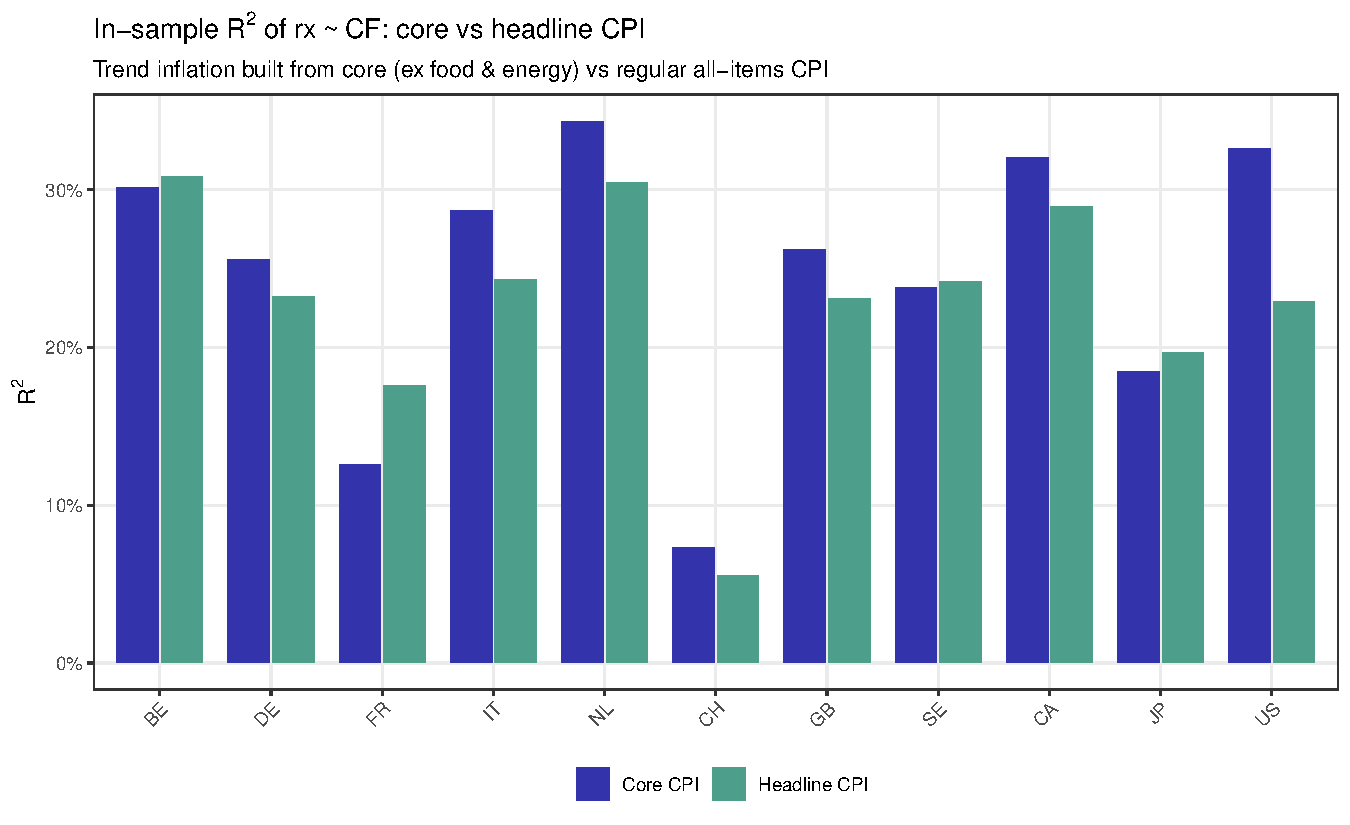
\includegraphics[width=0.88\linewidth]{figures/rob_f3_core_vs_reg.pdf}
  \caption{In-sample $R^{2}$ of the local predictive regression
    $\rxbar_{i,t+12}\sim\CF_{i,t}$ by country, with the cycle factor built on core
    (ex food and energy) versus regular all-items CPI.}
  \label{fig:rob-core-headline}
\end{figure}

\begin{figure}[htbp]\centering
  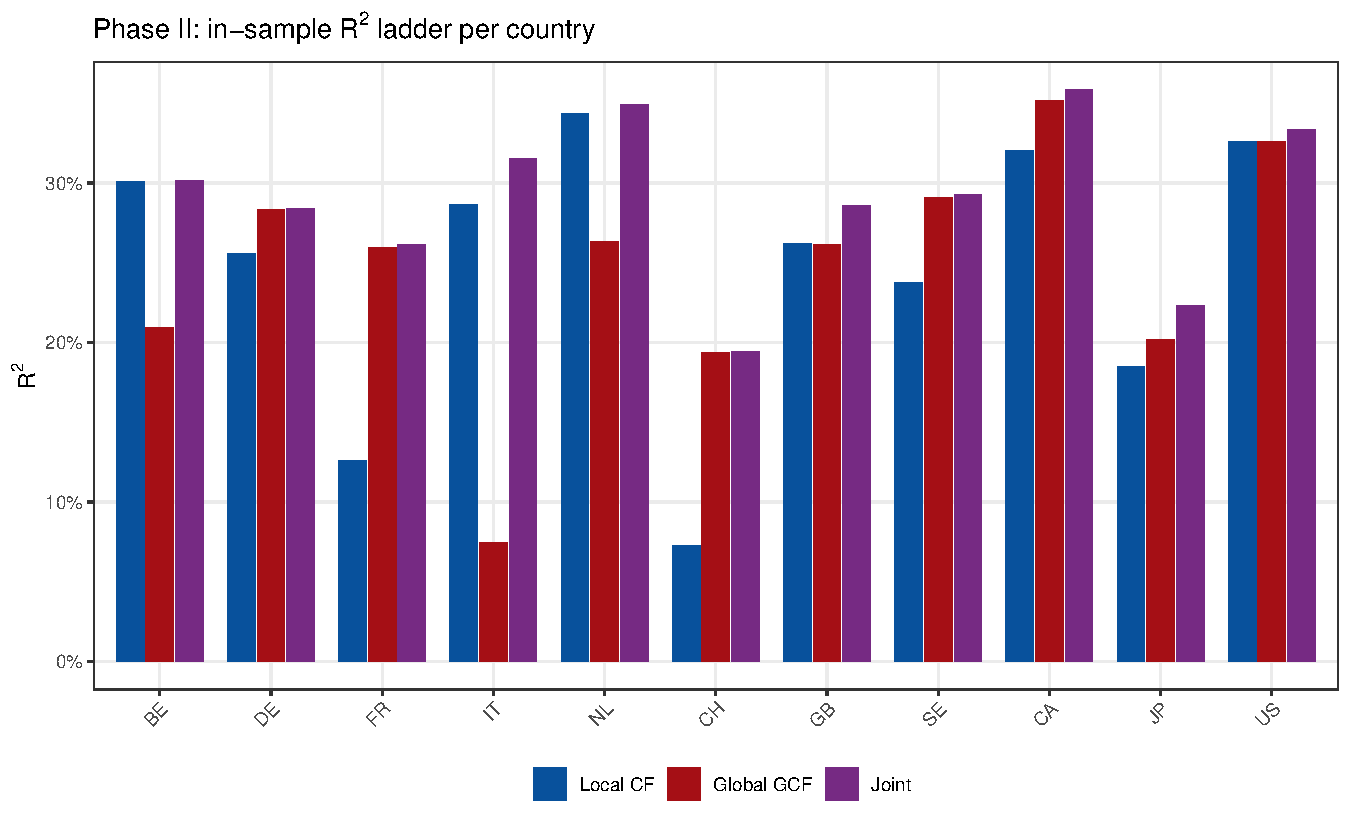
\includegraphics[width=0.9\linewidth]{figures/mr_f2_r2_ladder.pdf}
  \caption{Phase~II in-sample $R^{2}$ ladder by country: the local factor alone
    \eqref{eq:h-local}, the global factor alone \eqref{eq:h-global}, and the
    joint horse race \eqref{eq:h-horse}.}
  \label{fig:mr-r2-ladder}
\end{figure}

\begin{figure}[htbp]\centering
  
\includegraphics[width=0.9\linewidth]{figures/s1_yield_ts.pdf}
  \caption{Ten-year zero-coupon yields across the G10, 1989--2026. The secular
    decline in nominal yields and the post-2021 reversal are common across
    countries.}
  \label{fig:yield-ts}
\end{figure}

\begin{figure}[htbp]\centering
  \begin{minipage}[t]{0.49\linewidth}\centering
    
\includegraphics[width=\linewidth]{figures/s8_gcf_oos_vs_is.pdf}
  \end{minipage}\hfill
  \begin{minipage}[t]{0.49\linewidth}\centering
    
\includegraphics[width=\linewidth]{figures/s8_oos_is_corr.pdf}
  \end{minipage}
  \caption{Left: the full-sample global cycle factor $\GCF_{t}$ against the
    fully-recursive $\GCF^{\mathrm{oos}}_{t}$; convergence after the trend-inflation
    burn-in signals a stable real-time estimator. Right: per-country correlation
    between the full-sample and recursive \emph{local} cycle factors, where a
    value closer to one means that the full-sample look-ahead added little.}
  \label{fig:s8-gcf-conv}
\end{figure}

\section{AI Disclaimer}
\label{app:ai}
% Honest account of the AI-assisted tools used in this work. Keep this
% consistent with the "Statement on the use of generative AI tools" in the
% Declaration of Authorship.

In the preparation of this work, we used the following AI-assisted language and
coding models: Claude (Sonnet~4.6 and Opus~4.8, Anthropic) and ChatGPT Codex
(Codex~5.3 and GPT~5.5, OpenAI).

We used Claude and ChatGPT Codex to support the implementation of the coding
pipeline, including code generation and debugging, the validation of model
outputs, the summarisation of results, and the production of charts and
figures.

Additionally, ChatGPT Codex served as the execution environment for running
the code pipeline. We also used Claude in a minor supporting capacity during
the preparation of the presentation slides. However, all slides were conceived,
structured, and finalised by the human author, and the AI assistance represents
a negligible share of the final content.

All AI-generated outputs were reviewed, critically assessed, and adapted by the
author. We performed the data handling and model analysis locally. Model
training and index construction were implemented via cloud computing
(Vast.ai and GCP).
